%%%%%%%%%%%%%%%%%%%%%%%%%%%%%%%%%%%%%%%%%%%%%%%%%%%%%%%%%%%%%%%%%%%%%%%%%%%%%%%%%%%%%%%%%%%%%%%%%%%
%
%   Máster Universitario en Ciencia de Datos (MUCD)
%   Template for APPSIV labs
%   Author: Álvaro García Martín
%
%%%%%%%%%%%%%%%%%%%%%%%%%%%%%%%%%%%%%%%%%%%%%%%%%%%%%%%%%%%%%%%%%%%%%%%%%%%%%%%%%%%%%%%%%%%%%%%%%%%

\documentclass[letterpaper, 10 pt, conference]{IEEEtran}

% The following packages can be found on http:\\www.ctan.org
\usepackage{graphics} % for pdf, bitmapped graphics files
\usepackage{epsfig} % for postscript graphics files
\usepackage{mathptmx} % assumes new font selection scheme installed
\usepackage{times} % assumes new font selection scheme installed
\usepackage{amsmath} % assumes amsmath package installed
\usepackage{amssymb}  % assumes amsmath package installed
\usepackage{hyperref}
\usepackage{minted}
\usepackage[caption=false,font=footnotesize]{subfig}

\hypersetup{
  colorlinks=true,
  linkcolor=magenta,
  citecolor=magenta,
  pdfauthor={Antonio Coín},
  pdftitle={Lab 2 report},
  pdflang={English}
}

\title{\LARGE \bf Lab 2: Video classification}

\author{Antonio Coín Castro\\ \today}
\date{\today}
\begin{document}

\maketitle
\thispagestyle{plain} %--to force page numbers
\pagestyle{plain}


%%%%%%%%%%%%%%%%%%%%%%%%%%%%%%%%%%%%%%%%%%%%%%%%%%%%%%%%%%%%%%%%%%%%%%%%%%%%%%%%
\section{INTRODUCTION}
This report covers the work done for the video classification assignment. A series of experiments are carried out, in which the objective is to learn a function $f:\mathcal X\to \mathcal C$, where $\mathcal X=\{x_1,\dots, x_N\}$ is the labeled training set consisting on video frames, and $\mathcal C = \{C_1,\dots, C_K\}$ is the target class set (both $N$ and $K$ vary throughout the different experiments). The learned function is expected to approximate the genuine correspondence function that assigns every frame to its true class.
Two baseline methods are studied, namely the random and fixed mode classifiers, and then a third CNN-based classifier is presented, which is shown to greatly outperform the other two in terms of accuracy. Lastly, a thorough study of the performance of the CNN classifier is done with increasing quantities of samples and classes, analyzing the evolution of the learning curves and concluding that it performs well even on harder problems.


%%%%%%%%%%%%%%%%%%%%%%%%%%%%%%%%%%%%%%%%%%%%%%%%%%%%%%%%%%%%%%%%%%%%%%%%%%%%%%%%
\section{METHODS AND IMPLEMENTATION}
\label{sec:method}

In this section the methods employed in the experiments are briefly described, along with a general outline of their implementation. They can be run via the file \texttt{video\_classification.py}, or alternatively using the Jupyter notebook with the same name\footnote{The originally provided Python scripts have been slightly modified to better integrate them in the Jupyer notebook, as well as to allow the use of various versions of the data without preprocessing them differently.}. The only user-modifiable parameter is the variable \texttt{TRAIN\_CNN}, which controls whether the trainable models should be re-trained. If the models are indeed re-trained, the appropriate logs and checkpoints should also be specified in the code to view the corresponding results.
\subsection{Random mode classifier}

The first method implemented is the random classification algorithm. This is a method that simply assigns a random class to each video frame, that is, the function ``learned'' by this classifier is actually a random variable with uniform distribution over the classes: \[
f_R(x) \sim \text{Uniform}(\mathcal C).\]

Note that this is not a real classifier, but only a dummy method to set a baseline for further comparison; any decent classifier should outperform the random mode classifier in general. The implementation itself is trivial using the \texttt{random} library, and is available through the function \texttt{random\_vs\_fixed()} in the script \texttt{random\_vs\_fixed\_mode.py}.

\subsection{Fixed mode classifier}

The next algorithm is another baseline method that always assigns every frame to the same fixed class. Thus, it will always guess correctly the examples corresponding to the fixed class in question, but will fail to classify the rest of the frames. After fixing a desired class $C_k$, the underlying learned function is
\[
f_k(x) = C_k \quad \forall x \in \mathcal X.
\]

The code is present in the same function as the Random method, which runs both algorithms at once.

\subsection{CNN frame-by-frame classifier}

Lastly, a frame-by-frame classifier that is neither random nor fixed is implemented; one that actually takes into account the image features, and from which a good performance is expected. For this task, a pre-trained version of the \textit{InceptionV3} architecure \cite{inception} with Imagenet weights is used. This is a famous \textit{convolutional neural network} (CNN), widely and succesfully used for image classification tasks. A \textit{fine-tuning} approach is taken, in which the top layers of the pre-trained network are discarded and substituted for a fully-connected classifier. Then, firstly only the newly added layers are trained for a few epochs (to avoid distorting the network with random weights), and then some of the mid-top layers are unfrozen to perform the actual weight tuning. The rationale behind this decision is that the low-level features of the images in Imagenet are probably universal, and only the top layers of the network learn high-level distinctive features related to a particular problem.

From an implementation point of view, the \texttt{Keras} deep learning library \cite{keras} is used, which has an user-friendly and intuitive interface through its Model API. The code to train the CNN is available in the file \texttt{train\_cnn.py}, and the \texttt{get\_model()} function is the one that actually builds the model:

\begin{minted}{Python}
  base_model = InceptionV3(
      weights=weights,
      include_top=False)
  x = base_model.output
  x = GlobalAveragePooling2D()(x)
  x = Dense(1024, activation='relu')(x)
  predictions = Dense(
      nb_classes,
      activation='softmax')(x)
  model = Model(
      base_model.input,
      predictions,
      name="InceptionV3-finetune")
\end{minted}

As the code snippet shows, a standard fully connected layer with 1024 units is added on top of the pre-trained network, and then another one with $K$ units and softmax activation is appended. Note that some kind of global aggregation is needed before the dense layers, since the output of the base model is a 3-dimensional array. Instead of simply flattening said array, a global average pooling operation is performed, wich takes the average of each channel of the image (and thus carries out a significant dimensionality reduction). The output of the whole network is a $K$-dimensional vector, with each component representing the estimated probability that the processed image sample belongs to each class, which is denoted by $\tilde p(C_k\mid x)$. Then, the corresponding assignment is done by selecting the most likely outcome:
\[
f_{\text{Inception}}(x) = \arg \max_{C\in\mathcal C} \ \tilde p(C\mid x).
\]

After training the models they are evaluated using the functions available in the files \texttt{plot\_train\_cnnlog.py} and \texttt{validate\_cnn.py}.

%%%%%%%%%%%%%%%%%%%%%%%%%%%%%%%%%%%%%%%%%%%%%%%%%%%%%%%%%%%%%%%%%%%%%%%%%%%%%%%%
\section{EXPERIMENTAL METHODOLOGY}
\label{sec:methodology}

In this section an overview of the methodology followed is presented, focusing on the data used, the experiments performed and the evaluation metrics considered.
\subsection{Data}

For this assignment a subset of the UCF-101 action recognition dataset \cite{ucf} is considered. The videos are preprocessed to extract a number of frames from each one of them using the provided Python scripts, and then the image frames can be accessed via the \texttt{DataSet} class present in the \texttt{data.py} module. Specifically, four different versions of the data using $K\in\{5,10,15,20\}$ are considered, with 5 frames per video. Moreover, for the CNN models a train/validation split of roughly 70/30 is employed. A summary of the global data distribution can be seen on Table \ref{tab:data}, and further inspection reveals that the data is approximately balanced among all classes.

\begin{table}[h!]
  \centering
  \begin{tabular}{c|ccc}
    No. of classes & Train & Validation & Total\\
    \hline
    5 & 9490 & 3909 & 13399\\
    10 & 18452 & 6851 & 25303\\
    15 & 30147 & 11130 & 41277\\
    20 & 42245 & 16222 & 58467
  \end{tabular}\vspace{1em}
  \caption{Global image frames distribution}
  \label{tab:data}
\end{table}

In the case of the CNN models, data augmentation is also performed using random transformations at training time.

\subsection{Experiments}
\label{subsec:experiments}

For the first task, the performance of the random and fixed classifiers is compared by evaluating them on all available images using only $K=5$ classes, since they do not require any training whatsoever. In the case of the random classifier, 1000 independent runs of the experiment are performed to increase the stability of the results.

For the second task, the CNN model is trained on the same 5 classes and the results are compared to those of the fixed and random classifiers. As mentioned in Section \ref{sec:method}, the CNN training is performed in two steps. Firstly, only the top layers are trained for 10 epochs using the RMSProp optimizer. Then the last 172 layers of the network are unfrozen (using their \texttt{trainable} attribute) and the model is trained until an early stopping point is reached (specifically, when the validation loss does not decrease for 10 consecutive epochs), using the SGD optimizer with a reduced learning rate.

Finally, for the third task the performance of the CNN models on all four available data versions is studied, repeating the training each time with the appropriate parameters.

\subsection{Evaluation metrics}

The main evaluation metric considered is the \textit{accuracy} of the classifiers (abbreviated Acc), that is, the proportion of correctly classified samples over the total evaluation image frames. In addition, in the case of the CNN models a secondary metric is studied, namely the evolution of the categorical cross-entropy loss function over the epochs, both in training and validation sets.


%%%%%%%%%%%%%%%%%%%%%%%%%%%%%%%%%%%%%%%%%%%%%%%%%%%%%%%%%%%%%%%%%%%%%%%%%%%%%%%%
\section{RESULTS AND ANALYSIS}

In this section the results of the different experiments are presented and analyzed.

\subsection{Random vs. fixed mode}

Starting with the random classifier, the results in terms of accuracy on all runs are summarized on Table \ref{tab:random}.

\begin{table}[h!]
  \centering
  \begin{tabular}{c|cccc}
    & Min. & Max. & Median & Mean\\
    \hline
    Acc (\%) & 15.22 & 25.31 & 20.03 & 20.02
  \end{tabular}\vspace{1em}
  \caption{Statistical information after 1000 runs of the random classifier}
  \label{tab:random}
\end{table}

As the results show, the mean and median values are quite close, so the random classifier is stable and it can be stated that its accuracy is $20\%$. But this was surely to be expected, since that is precisely the expected value of the accuracy of the underlying uniform random variable after setting $K=5$:

\begin{equation}
  \label{eq:expectation}
\mathbb E\left[\operatorname{Acc}(f_R)\right] = \frac{1}{K}.
\end{equation}

On the other hand, the results for the fixed mode classifiers are shown on Table \ref{tab:fixed}, which contains one column for each fixed class: ApplyEyeMakeup (AEM), ApplyLipstick (AL), Archery (A), BabyCrawling (BC) and BalanceBeam (BB). In this mode there is no randomness involved, and the accuracy in each case is exactly the proportion of samples of the fixed reference class.

\begin{table}[h!]
  \centering
  \begin{tabular}{c|ccccc}
    & AEM & AL & A & BC & BB\\
    \hline
    Acc (\%) & 22.52 & 17.70 & 22.52 & 20.50 & 16.77
  \end{tabular}\vspace{1em}
  \caption{Accuracy for each of the fixed mode classifiers}
  \label{tab:fixed}
\end{table}

In addition, the class distribution of the samples is depicted in Figure \ref{fig:class_dist}, which confirms that higher accuracy values correspond to more density of samples of the fixed class in question.

\begin{figure}[h!]
  \centering
  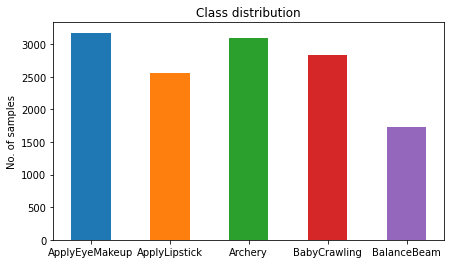
\includegraphics[width=.4\textwidth]{img/s1_class_distribution}
  \vspace{-.5em}
  \caption{Class distribution of the data with $K=5$.}
  \label{fig:class_dist}
\end{figure}

Finally, a side-to-side accuracy comparison of fixed vs. random mode is shown in Figure \ref{fig:comp_s1}, where it can be seen that the random mode beats some of the fixed mode classifiers, but also loses to others. All in all, they are quite similar and the differences are only due to the distribution of samples among the classes, in the sense that neither of them considers any kind of image features to perform the classification. As a matter of fact, it is easy to realize that the average of all the fixed mode classifiers corresponds to the average result of the random classifier, both theoretically and in practice. As stated before, these classifiers are not intended to be competitive, but only to set a reference baseline for evaluating the performance of other classifiers. As a general rule, if the random classifier performed noticeably better (or worse) than any of the fixed mode classifiers, it would be an indicative of an imbalanced distribution.

\begin{figure}[h!]
  \centering
  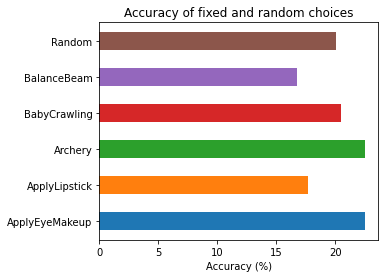
\includegraphics[width=.4\textwidth]{img/s1_accs}
  \vspace{-.5em}
  \caption{Accuracy of random and fixed mode classifiers with $K=5$.}
  \label{fig:comp_s1}
\end{figure}

\subsection{Random vs. fixed vs. CNN classifier}

In this experiment the frame-by-frame CNN model was trained with the data from $K=5$ classes following the procedure outlined in Section \ref{subsec:experiments}. The early stopping point in the second step of the training phase turned out to be 18 epochs, and the corresponding training and validation accuracy curves can be seen in Figure \ref{fig:acc5}. It is eminently clear that this model vastly outperforms the random and fixed mode classifiers, reaching an accuracy of over 90\% in both training and validation sets. However, the associated computational cost is also higher, since it takes about 15 minutes to execute on a GPU in Google Colab while the baseline models finish almost instantly\footnote{The execution times might not be entirely faithful, because Colab takes an artificially long time to process files from the connected Drive directory.}.

\begin{figure}[t]
  \centering
  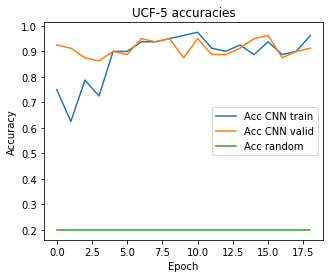
\includegraphics[width=.35\textwidth]{img/ucf5-acc}
  \vspace{-.5em}
  \caption{Accuracy curves of CNN classifier with $K=5$.}
  \label{fig:acc5}
\end{figure}

\subsection{CNN classifier with different number of classes}

A last experiment is performed in which the number of video classes and image samples is increased little by little, ranging from the initial 5 classes all the way up to 20 classes, with a step size of 5 (see Table \ref{tab:data} above). The resulting accuracy curves can be seen in Figure \ref{fig:acc_comparison}, which show that the higher the number of classes, the harder the problem, and the more difficult is for the network to obtain good results. The expected accuracy of the random classifier is also shown in the plot for reference (as defined in Eq. \ref{eq:expectation}).

Moreover, Figure \ref{fig:loss_comparison} depicts the evolution of the loss curves for each model. An immediate observation is that the initial value of the loss function gets higher as the number of classes increases, and overall the final loss value is also higher, but it does decrease over time. As the analogous phenomenon is observed in the accuracy curves, it can therefore be concluded that the network is learning correctly, but the problem is getting harder each time. The execution time also reflects this behaviour, since it increases accordingly with each new model. Note that the number of training epochs is roughly the same for every model, and because of the early stopping technique, they would most likely not benefit from further training.

The fact that the validation accuracy is generally higher than the training accuracy (and the validation loss lower than the training loss) shows that the model has learned to generalize well to previously unseen images, probably due to the adequacy of the model to the data and the suite of regularization techniques employed under the hood.

\begin{figure*}[t]
     \centering
     \subfloat{
         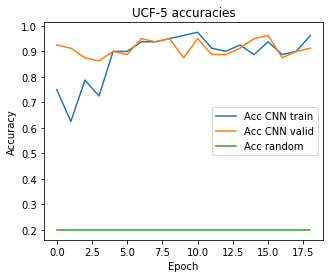
\includegraphics[width=.32\textwidth]{img/ucf5-acc}}
     \subfloat{
         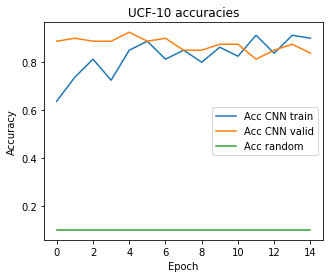
\includegraphics[width=.32\textwidth]{img/ucf10-acc}}
     \\
     \subfloat{
         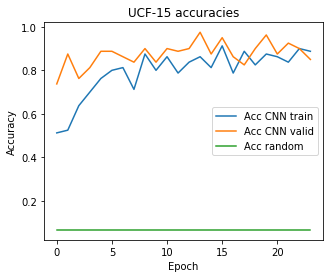
\includegraphics[width=.32\textwidth]{img/ucf15-acc}}
     \subfloat{
         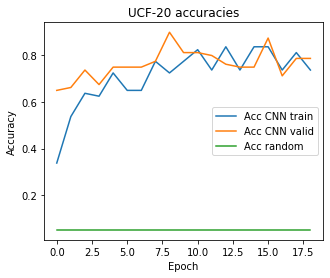
\includegraphics[width=.32\textwidth]{img/ucf20-acc}}
        \caption{Accuracy curves for all versions of the CNN classifier ($K=5,10,15,20$).}
        \label{fig:acc_comparison}
\end{figure*}

\begin{figure*}[h!]
     \centering
     \subfloat{
         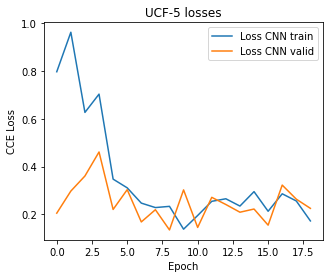
\includegraphics[width=.32\textwidth]{img/ucf5-loss}}
     \subfloat{
         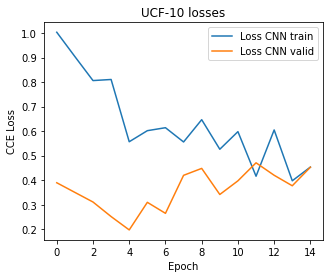
\includegraphics[width=.32\textwidth]{img/ucf10-loss}}
     \\
     \subfloat{
         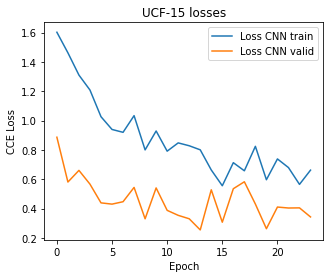
\includegraphics[width=.32\textwidth]{img/ucf15-loss}}
     \subfloat{
         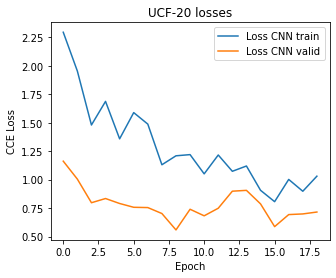
\includegraphics[width=.32\textwidth]{img/ucf20-loss}}
        \caption{Loss curves for all versions of the CNN classifier ($K=5,10,15,20$).}
        \label{fig:loss_comparison}
\end{figure*}

Even though the model performs well, there are still some images that it gets wrong by a large margin. For example, in Figure \ref{fig:example} there is a selection of two images fed to the 5-class CNN model for prediction. The leftmost image is correctly classified by the network in the ApplyLipstick class, whereas the rightmost image is wrongly given a 0.78 probability of belonging to the same ApplyLipstick class. This is probably due to the partial occlusion of the lips and the similarity of the pose to the act of applying lipstick. In fact, these are generally the traits that are challenging for CNNs to differentiate, and our relatively simple model is no exception.

\begin{figure}[h!]
    \centering
     \subfloat[ApplyLipstick]{
         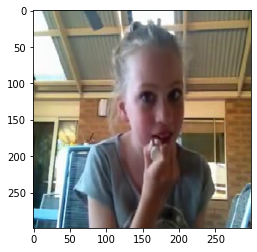
\includegraphics[width=.23\textwidth]{img/ex1}}
     \subfloat[ApplyEyeMakeup]{
         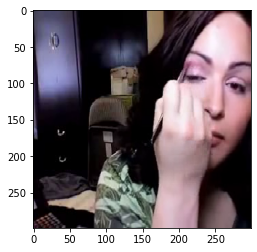
\includegraphics[width=.23\textwidth]{img/ex2}}
    \caption{Two images of the UCF-5 subset.}
    \label{fig:example}
\end{figure}

%%%%%%%%%%%%%%%%%%%%%%%%%%%%%%%%%%%%%%%%%%%%%%%%%%%%%%%%%%%%%%%%%%%%%%%%%%%%%%%%
\section{CONCLUSIONS}

In conclusion, a properly built frame-by-frame CNN classifier greatly outperforms the random and fixed mode baseline classifiers (which are themselves quite similar), and even more so when the number of classes increases and the problem gets more difficult. However, the improvement in accuracy comes at the expense of a greater computational time, which can sometimes be prohibitive if the problem at hand is big and one does not have the appropriate hardware and software resources.

In the case of 20 classes the accuracy of the CNN model starts falling below the 80\% threshold, which indicates that it is still not powerful and flexible enough to handle bigger-sized and more realistic problems. Although the frame-by-frame approach works sufficiently well for the data used in this assignment, it is likely that more sophisticated and specific methods for video handling would need to be used to obtain good results in harder settings. For example, a fairly comprehensive survey on human activity video recognition is \cite{survey}, in which the authors explore the different techniques that emerged over the last decade with emphasis on deep learning models.

%%%%%%%%%%%%%%%%%%%%%%%%%%%%%%%%%%%%%%%%%%%%%%%%%%%%%%%%%%%%%%%%%%%%%%%%%%%%%%%%
\begin{thebibliography}{99}

\bibitem{inception} Szegedy, C., Vanhoucke, V., Ioffe, S., Shlens, J., \& Wojna, Z. (2016). Rethinking the inception architecture for computer vision. In \textit{Proceedings of the IEEE conference on computer vision and pattern recognition} (pp. 2818-2826).
\bibitem{keras} Chollet, F. et al. (2015). Keras. \url{https://keras.io}.

\bibitem{ucf} Soomro, K., Zamir, A. R., \& Shah, M. (2012). UCF101: A dataset of 101 human actions classes from videos in the wild. \textit{arXiv preprint arXiv:1212.0402}. \url{https://www.crcv.ucf.edu/data/UCF101.php}.

\bibitem{survey} Herath, S., Harandi, M., \& Porikli, F. (2017). Going deeper into action recognition: A survey. \textit{Image and vision computing}, 60, 4-21.
\end{thebibliography}


%%%%%%%%%%%%%%%%%%%%%%%%%%%%%%%%%%%%%%%%%%%%%%%%%%%%%%%%%%%%%%%%%%%%%%%%%%%%%%%%
\appendix

\subsection{TIME LOG}

The approximate time spent on each task is summarized below.

\begin{itemize}
  \item \textit{Reading and understanding the code:} 30 min.
  \item \textit{Preparing the environment and the data, and modifying the scripts to fit our needs}: 1h 30 min.
  \item \textit{Experiments}: 2h (mostly idle running the code).
  \item \textit{Report}: 4h (including drafting, revising and correcting errors).
\end{itemize}

\end{document}
